\begin{frame}
    \frametitle{Testing}
    
    \begin{multicols}{2}
        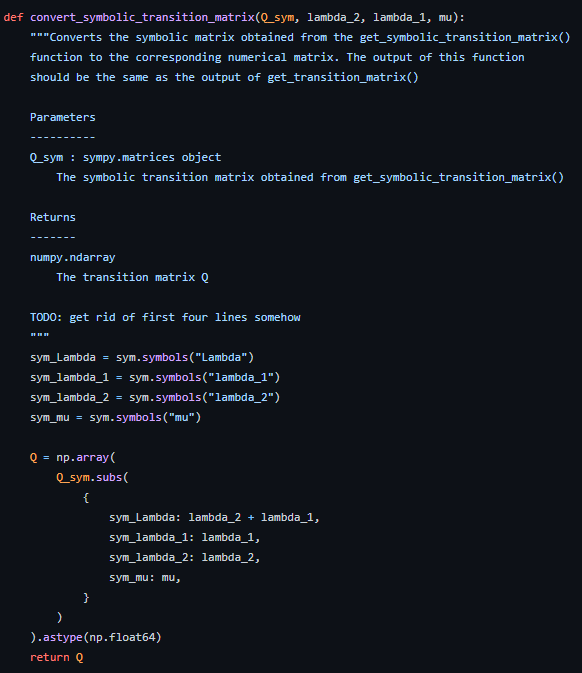
\includegraphics[width=0.48\textwidth]{Bin/ambulance_game_code.PNG}

        \columnbreak

        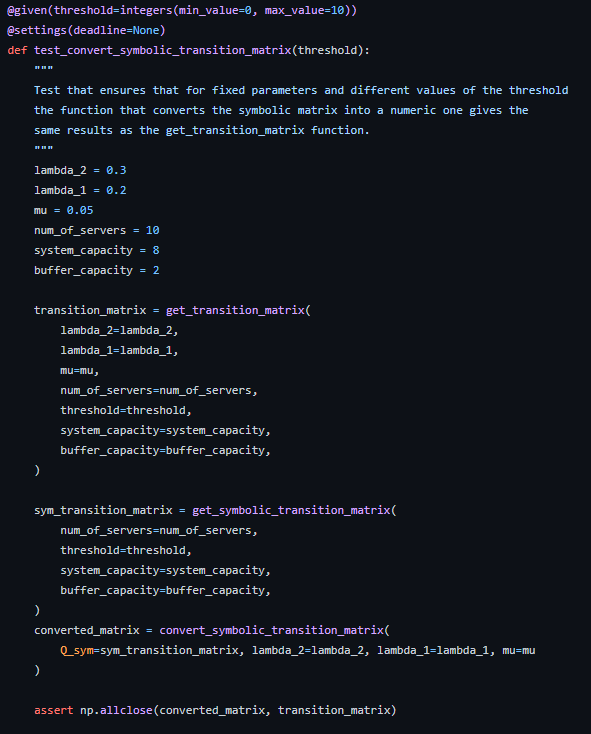
\includegraphics[width=0.48\textwidth]{Bin/ambulance_game_test.PNG}
    \end{multicols}

\end{frame}


\begin{frame}
    \frametitle{Linters}
    \centering

    \textit{Linting} is the automated checking of your source code for 
    programmatic and stylistic errors without running the code
    
    \vspace{1cm}

    Linting tools:
    
    \begin{multicols}{3}
        \begin{itemize}
            \item black
            \item pylint
            \item tox
            \item flake8
            \item mccabe
            \item mypy
        \end{itemize}
    \end{multicols}
\end{frame}


\begin{frame}
    \frametitle{GitHub Actions}

    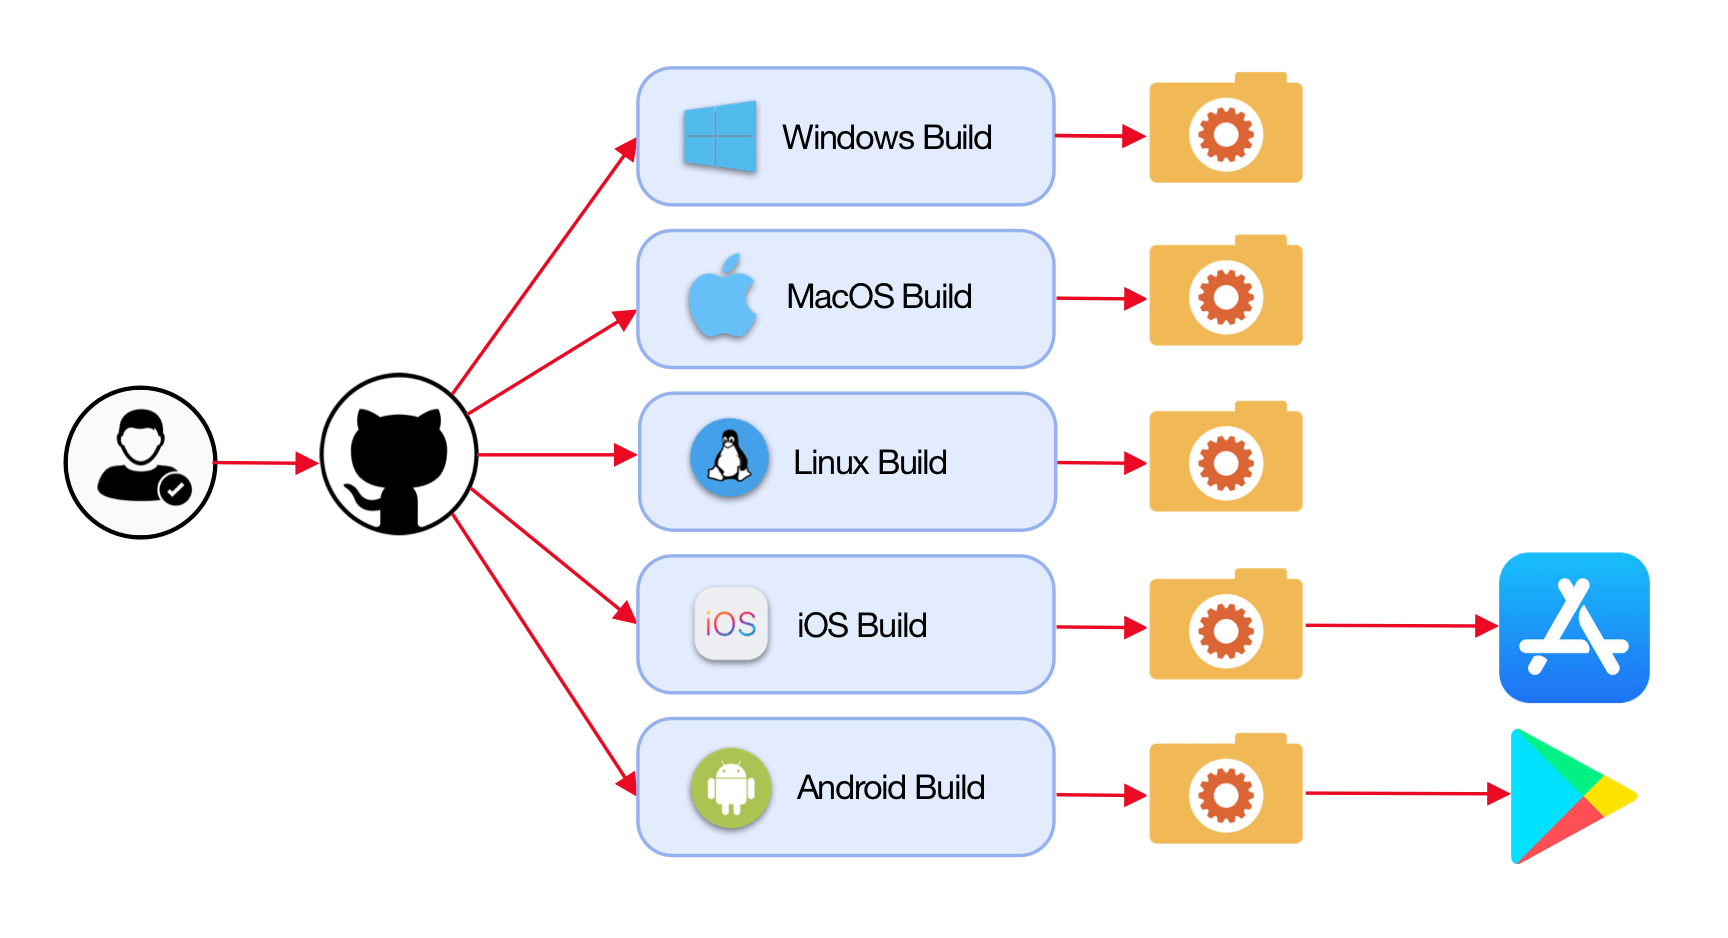
\includegraphics[width=\textwidth]{Bin/github_actions.png}

\end{frame}

